\documentclass{article}
\usepackage{tikz,amsmath,siunitx}
\usepackage{pgfplots}
\usepackage{listings}
\usetikzlibrary{arrows,snakes,backgrounds,patterns,matrix,shapes,fit,calc,shadows,plotmarks}
\topmargin -1.5cm        % read Lamport p.163
\oddsidemargin -0.04cm   % read Lamport p.163
\evensidemargin -0.04cm  % same as oddsidemargin but for left-hand pages
\textwidth 16.59cm
\textheight 21.94cm 
%\usepackage[graphics,tightpage,active]{preview}
%\PreviewEnvironment{tikzpicture}
%\PreviewEnvironment{equation}
%\PreviewEnvironment{equation*}
\title{CS540 Assignment 2}
\author{Dustin Ingram}
\newlength{\imagewidth}
\newlength{\imagescale}
\pagestyle{empty}
\thispagestyle{empty}
\lstset{breaklines=true}
\begin{document}
\maketitle
\newpage
\section{Introduction}
For this assignment, various methods of mini- matrix multiplication are compared, including matrix blocking and loop unrolling. The results are compared based on the performance to determine the optimal block size for a particular system.
\section{Summary of Results}
The results can be organized as follows:
\subsection{Blocking, Unrolling, and Scalar Replacement}
It was found that blocking the matrix, unrolling the innermost loop, and performing scalar replacement and addition/subtraction interleaving greatly improved performance. 
\subsection{Loop Ordering}
It was found that differences in loop ordering produced results that were essentially the same, thereby offering no improvement in performance.
\subsection{Matrix Size Comparisons}
As expected, it was found that the best implementation with the highest-performing values for block size performed better than the na\"{\i}ve code.
\section{Description of Computing Platform}
All tests were run on \texttt{float.cs.drexel.edu}. Relevant system architecture information follows.
\subsection{System \& Kernel Information}
\begin{lstlisting}
$ uname -a
Linux float.cs.drexel.edu 2.6.35-28-generic #50-Ubuntu SMP Fri Mar 18 18:42:20 UTC 2011 x86_64 GNU/Linux
\end{lstlisting}
\subsection{GCC Version Information}
\begin{lstlisting}
$ gcc --version
gcc (Ubuntu/Linaro 4.4.4-14ubuntu5) 4.4.5
\end{lstlisting}
\subsection{CPU Information}
\begin{lstlisting}
$ cat /proc/cpuinfo
processor	: 15
vendor_id	: GenuineIntel
cpu family	: 6
model		: 44
model name	: Intel(R) Xeon(R) CPU           L5630  @ 2.13GHz
stepping	: 2
cpu MHz		: 1600.000
cache size	: 12288 KB
physical id	: 1
siblings	: 8
core id		: 10
cpu cores	: 4
apicid		: 53
initial apicid	: 53
fpu		: yes
fpu_exception	: yes
cpuid level	: 11
wp		: yes
flags		: fpu vme de pse tsc msr pae mce cx8 apic sep mtrr pge mca cmov pat pse36 clflush dts acpi mmx fxsr sse sse2 ss ht tm pbe syscall nx pdpe1gb rdtscp lm constant_tsc arch_perfmon pebs bts rep_good xtopology nonstop_tsc aperfmperf pni pclmulqdq dtes64 monitor ds_cpl vmx smx est tm2 ssse3 cx16 xtpr pdcm dca sse4_1 sse4_2 popcnt aes lahf_lm ida arat dts tpr_shadow vnmi flexpriority ept vpid
bogomips	: 4266.84
clflush size	: 64
cache_alignment	: 64
address sizes	: 40 bits physical, 48 bits virtual
power management:
\end{lstlisting}
\subsection{Memory Information}
\begin{lstlisting}
$ papi_mem_info
Memory Cache and TLB Hierarchy Information.
------------------------------------------------------------------------
TLB Information.
  There may be multiple descriptors for each level of TLB
  if multiple page sizes are supported.

L1 Instruction TLB:
  Page Size:           2048 KB
  Number of Entries:      7
  Associativity:       Full

L1 Instruction TLB:
  Page Size:           4096 KB
  Number of Entries:      7
  Associativity:       Full

L1 Data TLB:
  Page Size:              4 KB
  Number of Entries:     64
  Associativity:          4

L1 Data TLB:
  Page Size:           2048 KB
  Number of Entries:     32
  Associativity:          4

L1 Data TLB:
  Page Size:           4096 KB
  Number of Entries:     32
  Associativity:          4

L1 Instruction TLB:
  Page Size:              4 KB
  Number of Entries:     64
  Associativity:          4


Cache Information.

L1 Data Cache:
  Total size:            32 KB
  Line size:             64 B
  Number of Lines:      512
  Associativity:          8

L1 Instruction Cache:
  Total size:            32 KB
  Line size:             64 B
  Number of Lines:      512
  Associativity:          4

L2 Unified Cache:
  Total size:           256 KB
  Line size:             64 B
  Number of Lines:     4096
  Associativity:          8

L3 Unified Cache:
  Total size:         12288 KB
  Line size:             64 B
  Number of Lines:   196608
  Associativity:         16

mem_info.c                               PASSED
\end{lstlisting}

\newpage
\section{Experiments Performed \& Results}
\subsection{Optimations of Mini-MMM: Blocking, Unrolling, and Scalar Replacement}
Here the following implementations are compared for a range of block sizes such that $16\leq N_{B}\leq 80$, with 4 divides $N_{B}$.
\begin{itemize}
    \item \texttt{code0} -- the numerical recipes code;
    \item \texttt{code1} -- blocked into micro MMMs and unrolled;
    \item \texttt{code2} -- further unrolling; and
    \item \texttt{code3} -- even further unrolling.
\end{itemize}    

Since, in this comparison, the blocks and the matrices both have a size $N_{B}\times{N_{B}}$, the time to compute the MMM is not useful for determining a optimal $N_{B}$, therefore we must instead compare the performance of each block in terms of MFLOPs/sec.\\

\pgfplotsset{width=15cm,compat=1.4}
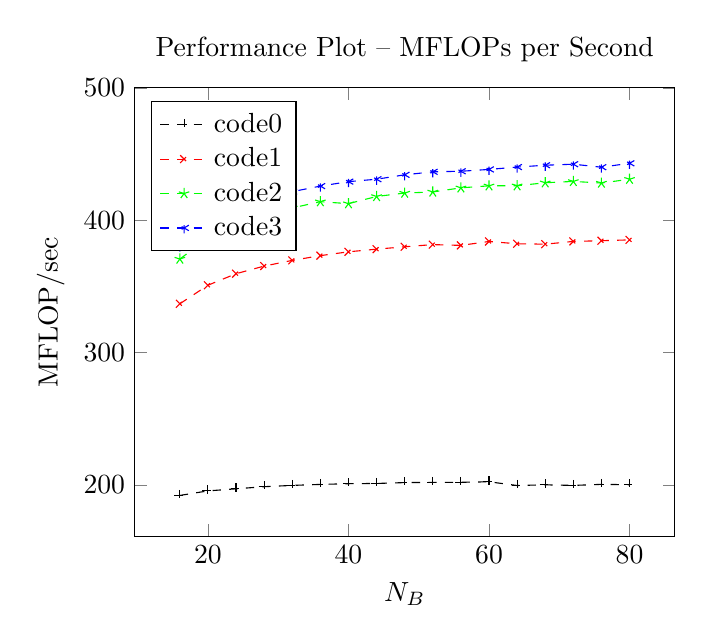
\begin{tikzpicture}
\begin{axis}[
ymax=500,
xlabel=$N_{B}$,
ylabel=MFLOP/sec,
legend pos=north west,
title=Performance Plot -- MFLOPs per Second] 
\legend{code0, code1, code2, code3}

\addplot[color=black,mark=+,dashed] coordinates {
(	16	,	192.0370934864	)
(	20	,	195.4690978022	)
(	24	,	197.035936102	)
(	28	,	198.6491305292	)
(	32	,	199.6154641715	)
(	36	,	200.3671516101	)
(	40	,	200.9016516226	)
(	44	,	201.0859597248	)
(	48	,	201.7429824469	)
(	52	,	201.884920757	)
(	56	,	201.9698063396	)
(	60	,	202.3419391736	)
(	64	,	199.5487589353	)
(	68	,	200.0462902639	)
(	72	,	199.6106650882	)
(	76	,	200.4031035144	)
(	80	,	200.1392676137	)
};

\addplot[color=red,mark=x,dashed] coordinates {
(	16	,	336.8424161184	)
(	20	,	350.8775339912	)
(	24	,	359.5790175576	)
(	28	,	365.349454606	)
(	32	,	369.6339176537	)
(	36	,	373.2334661814	)
(	40	,	376.1281151891	)
(	44	,	378.1254706365	)
(	48	,	379.9306817081	)
(	52	,	381.5689622524	)
(	56	,	380.9833876843	)
(	60	,	383.9355837236	)
(	64	,	382.1930559998	)
(	68	,	381.9009306418	)
(	72	,	383.9688043011	)
(	76	,	384.522342909	)
(	80	,	385.1409679175	)
};

\addplot[color=green,mark=star,dashed] coordinates {
(	16	,	370.6791149321	)
(	20	,	386.4738002415	)
(	24	,	397.0136680069	)
(	28	,	404.4592128052	)
(	32	,	409.2679140698	)
(	36	,	414.002845601	)
(	40	,	412.5045144054	)
(	44	,	417.9480945465	)
(	48	,	420.5263393159	)
(	52	,	421.34207424	)
(	56	,	424.4706101443	)
(	60	,	425.9855439199	)
(	64	,	426.0396517337	)
(	68	,	428.3090384199	)
(	72	,	429.3122785567	)
(	76	,	428.0922268474	)
(	80	,	430.9696415338	)
};

\addplot[color=blue,mark=asterisk,dashed] coordinates {
(	16	,	380.4928704134	)
(	20	,	397.7135356699	)
(	24	,	408.3301019052	)
(	28	,	416.1520905213	)
(	32	,	421.5893579286	)
(	36	,	425.7715443055	)
(	40	,	429.156230403	)
(	44	,	430.9736157193	)
(	48	,	434.2992071904	)
(	52	,	436.5628043343	)
(	56	,	436.9975008709	)
(	60	,	438.3699779902	)
(	64	,	440.1606572247	)
(	68	,	441.5440214641	)
(	72	,	442.318694944	)
(	76	,	440.0545829833	)
(	80	,	443.0087280389	)
};
\end{axis}
\end{tikzpicture}

Here, it is clear that \texttt{code3} outperforms all other implementations, and it appears that the optimal size for $N_{B}$ is $N_{B}=80$; however, since this is seemingly a completely arbitrary and baseless number, it cannot be taken for granted. 

\newpage
If one instead examines possible block sizes as large as $N_{B}=480$ and beyond, one sees that $N_{B}=80$ is not in fact the highest-performing block size.\\

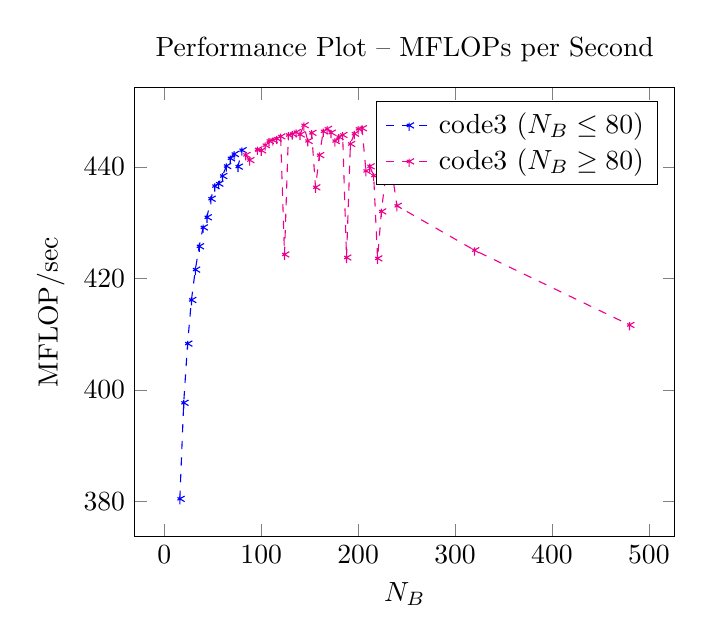
\begin{tikzpicture}
\begin{axis}[
xlabel=$N_{B}$,
ylabel=MFLOP/sec,
legend pos=north east,
title=Performance Plot -- MFLOPs per Second] 
\legend{code3 ($N_{B}\leq80$), code3 ($N_{B}\geq80$)}

\addplot[color=blue,mark=asterisk,dashed] coordinates {
(	16	,	380.4928704134	)
(	20	,	397.7135356699	)
(	24	,	408.3301019052	)
(	28	,	416.1520905213	)
(	32	,	421.5893579286	)
(	36	,	425.7715443055	)
(	40	,	429.156230403	)
(	44	,	430.9736157193	)
(	48	,	434.2992071904	)
(	52	,	436.5628043343	)
(	56	,	436.9975008709	)
(	60	,	438.3699779902	)
(	64	,	440.1606572247	)
(	68	,	441.5440214641	)
(	72	,	442.318694944	)
(	76	,	440.0545829833	)
(	80	,	443.0087280389	)
};

\addplot[color=magenta,mark=asterisk,dashed] coordinates {
(   84  ,   442.1534382693  )
(   88  ,   441.225549045   )
(   96  ,   443.1439874781  )
(   100 ,   442.9683975637  )
(   104 ,   443.9089017364  )
(   108 ,   444.6569890575  )
(   112 ,   444.8093267374  )
(   116 ,   445.0806023667  )
(   120 ,   445.4777009539  )
(   124 ,   424.3076639591  )
(   128 ,   445.7288862912  )
(   132 ,   445.9037272199  )
(   136 ,   446.2406754479  )
(   140 ,   445.8170916328  )
(   144 ,   447.4729689045  )
(   148 ,   444.6603504561  )
(   152 ,   446.1142916667  )
(   156 ,   436.3451024654  )
(   160 ,   442.1187203843  )
(   164 ,   446.3846701412  )
(   168 ,   446.8196931304  )
(   172 ,   446.1404260225  )
(   176 ,   444.6442720822  )
(   180 ,   445.3783548055  )
(   184 ,   445.7291220664  )
(   188 ,   423.7555829215  )
(   192 ,   444.1174035891  )
(   196 ,   445.9575109867  )
(   200 ,   446.8155023318  )
(   204 ,   446.9427361674  )
(   208 ,   439.2824869786  )
(   212 ,   440.1089719624  )
(   216 ,   438.4376655935  )
(   220 ,   423.5992076819  )
(   224 ,   432.0285855163  )
(   228 ,   437.8737051315  )
(   232 ,   439.5734166857  )
(   236 ,   437.7994733958  )
(   240 ,   433.0289685816  )
(   320 ,   425.0677350335  )
(   480 ,   411.6696131278  )
};
\end{axis}
\end{tikzpicture}

This reveals that peak performance is achieved at $N_{B}=144$. One can notice obviously large amounts of data cache misses at $N_{B}=\{124, 156, 188, 220\}$.

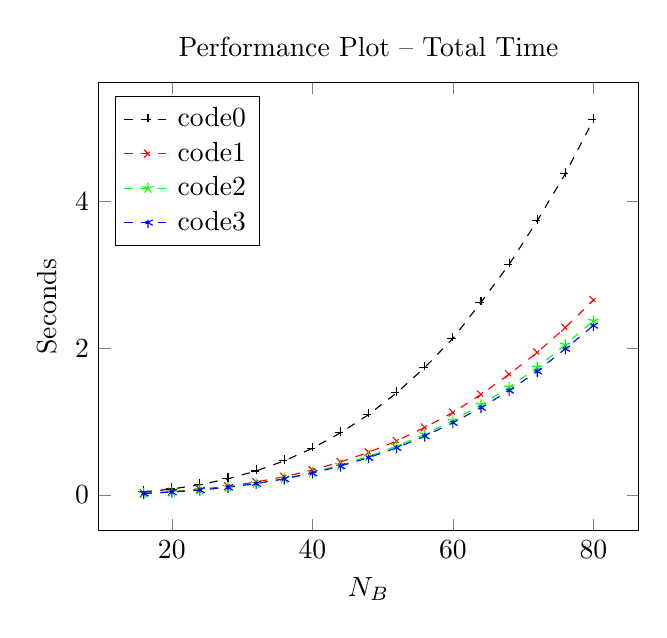
\begin{tikzpicture}
\begin{axis}[
xlabel=$N_{B}$,
ylabel=Seconds,
legend pos=north west,
title=Performance Plot -- Total Time] 
\legend{code0, code1, code2, code3}

\addplot[color=black,mark=+,dashed] coordinates {
(	16	,	0.04268	)
(	20	,	0.0819	)
(	24	,	0.14038	)
(	28	,	0.2211	)
(	32	,	0.32837	)
(	36	,	0.4658	)
(	40	,	0.63724	)
(	44	,	0.84742	)
(	48	,	1.09667	)
(	52	,	1.39331	)
(	56	,	1.73954	)
(	60	,	2.13542	)
(	64	,	2.62751	)
(	68	,	3.14376	)
(	72	,	3.73994	)
(	76	,	4.38113	)
(	80	,	5.11689	)
};

\addplot[color=red,mark=x,dashed] coordinates {
(	16	,	0.02432	)
(	20	,	0.0456	)
(	24	,	0.07689	)
(	28	,	0.12017	)
(	32	,	0.1773	)
(	36	,	0.25001	)
(	40	,	0.34031	)
(	44	,	0.45056	)
(	48	,	0.58217	)
(	52	,	0.737	)
(	56	,	0.92191	)
(	60	,	1.12519	)
(	64	,	1.37179	)
(	68	,	1.64667	)
(	72	,	1.94416	)
(	76	,	2.28323	)
(	80	,	2.65877	)
};

\addplot[color=green,mark=star,dashed] coordinates {
(	16	,	0.0221	)
(	20	,	0.0414	)
(	24	,	0.06964	)
(	28	,	0.10855	)
(	32	,	0.16013	)
(	36	,	0.22539	)
(	40	,	0.3103	)
(	44	,	0.40763	)
(	48	,	0.52597	)
(	52	,	0.66743	)
(	56	,	0.82746	)
(	60	,	1.01412	)
(	64	,	1.23061	)
(	68	,	1.46825	)
(	72	,	1.73882	)
(	76	,	2.05085	)
(	80	,	2.37604	)
};

\addplot[color=blue,mark=asterisk,dashed] coordinates {
(	16	,	0.02153	)
(	20	,	0.04023	)
(	24	,	0.06771	)
(	28	,	0.1055	)
(	32	,	0.15545	)
(	36	,	0.21916	)
(	40	,	0.29826	)
(	44	,	0.39531	)
(	48	,	0.50929	)
(	52	,	0.64416	)
(	56	,	0.80374	)
(	60	,	0.98547	)
(	64	,	1.19113	)
(	68	,	1.42424	)
(	72	,	1.68769	)
(	76	,	1.9951	)
(	80	,	2.31147	)
};
\end{axis}
\end{tikzpicture}

This plot gives an idea of how much faster each version is for various block sizes. There is a nice, smooth trend.

\newpage
\section{Loop Ordering}
When comparing the ordering of the outermost loop, it now becomes necessary to move beyond the performance of single-block matrices, to the performance of small blocks within larger matrices.\\

Since it is necessary that $N_{B}$ divides into the dimensions of the matrix, we must choose certain values. Selecting a reasonable set $S$ of block sizes and a reasonable sized $N\times{N}$ matrix such that \textsc{LeastCommonMultiple}$(S) = N$ gives $S=\{16,32,48,64,80,96,120,160,192,240,320,480,960\}$, and $N=960$.\\

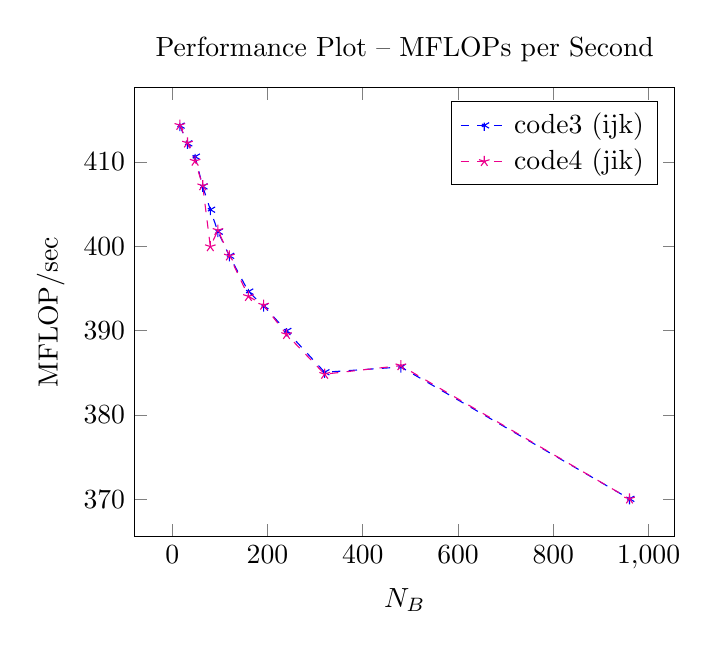
\begin{tikzpicture}
\begin{axis}[
xlabel=$N_{B}$,
ylabel=MFLOP/sec,
legend pos=north east,
title=Performance Plot -- MFLOPs per Second] 
\legend{code3 (ijk), code4 (jik)}

\addplot[color=blue,mark=asterisk,dashed] coordinates {
(   16  ,   414.3203232443  )
(   32  ,   412.2150194868  )
(   48  ,   410.6374966245  )
(   64  ,   407.1073105968  )
(   80  ,   404.3428213705  )
(   96  ,   401.7383241486  )
(   120 ,   398.8657011301  )
(   160 ,   394.6260192115  )
(   192 ,   392.9061387787  )
(   240 ,   389.9583425599  )
(   320 ,   385.0535182139  )
(   480 ,   385.6745839146  )
(   960 ,   370.0296453367  )
};

\addplot[color=magenta,mark=star,dashed] coordinates {
(   16  ,   414.3666028487  )
(   32  ,   412.2672794031  )
(   48  ,   410.1183681898  )
(   64  ,   407.1990463717  )
(   80  ,   399.9703296074  )
(   96  ,   401.9044539542  )
(   120 ,   398.8657283001  )
(   160 ,   394.0623712241  )
(   192 ,   393.0294547041  )
(   240 ,   389.5470998591  )
(   320 ,   384.8274188687  )
(   480 ,   385.8427621021  )
(   960 ,   370.0296746131  )
};
\end{axis}
\end{tikzpicture}

From this graph it appears that there is no performance increase as a result of the new loop ordering.

\newpage
It is possible to check the timing of these different implementations of loop order for a more definite answer. \\

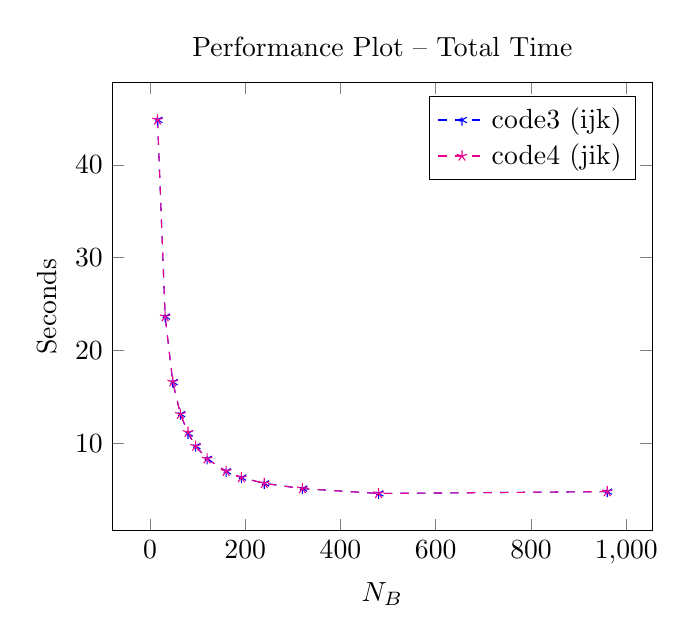
\begin{tikzpicture}
\begin{axis}[
xlabel=$N_{B}$,
ylabel=Seconds,
legend pos=north east,
title=Performance Plot -- Total Time] 
\legend{code3 (ijk), code4 (jik)}

\addplot[color=blue,mark=asterisk,dashed] coordinates {
(   16  ,   44.867  )
(   32  ,   23.657  )
(   48  ,   16.59   )
(   64  ,   13.136  )
(   80  ,   11.062  )
(   96  ,   9.69    )
(   120 ,   8.318   )
(   160 ,   6.975   )
(   192 ,   6.305   )
(   240 ,   5.672   )
(   320 ,   5.106   )
(   480 ,   4.588   )
(   960 ,   4.782   )
};

\addplot[color=magenta,mark=star,dashed] coordinates {
(   16  ,   44.862  )
(   32  ,   23.654  )
(   48  ,   16.611  )
(   64  ,   13.133  )
(   80  ,   11.183  )
(   96  ,   9.686   )
(   120 ,   8.318   )
(   160 ,   6.985   )
(   192 ,   6.303   )
(   240 ,   5.678   )
(   320 ,   5.109   )
(   480 ,   4.586   )
(   960 ,   4.782   )
};
\end{axis}
\end{tikzpicture}

There is clearly no difference between the loop orderings.

\newpage
\subsection{Matrix Size Comparisons}
Finally, one can compare the the performance of high-performing block sizes $N_{B}=\{80,144\}$ for a range of matrix dimensions $0 \leq N \leq 2400$.\\

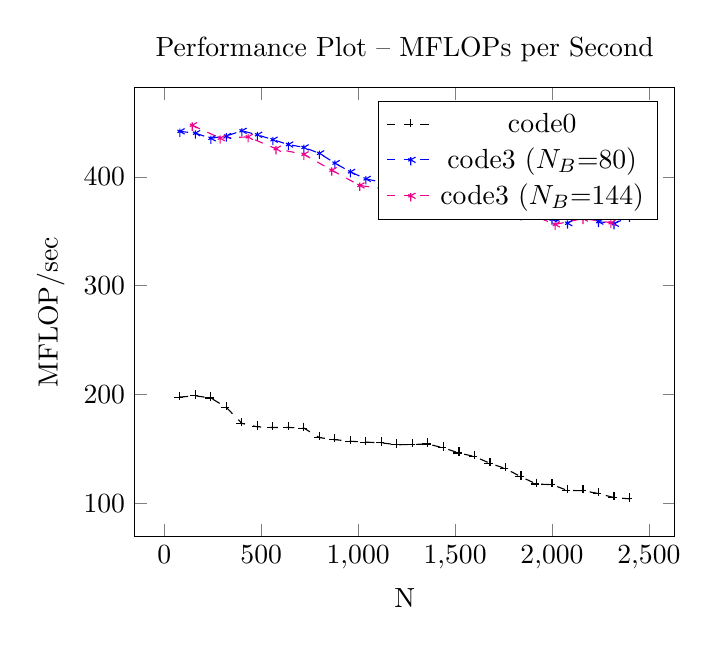
\begin{tikzpicture}
\begin{axis}[
xlabel=N,
ylabel=MFLOP/sec,
legend pos=north east,
title=Performance Plot -- MFLOPs per Second] 
\legend{code0, code3 ($N_{B}$=80), code3 ($N_{B}$=144)}

\addplot[color=black,mark=+,dashed] coordinates {
(	80	,	197.6929826255	)
(	160	,	198.8440728155	)
(	240	,	196.8224896797	)
(	320	,	188.1825815155	)
(	400	,	173.5493932539	)
(	480	,	170.3740100077	)
(	560	,	169.7130381458	)
(	640	,	169.8101313916	)
(	720	,	169.2183857305	)
(	800	,	160.4442840376	)
(	880	,	158.5767076941	)
(	960	,	157.1294912172	)
(	1040	,	156.300815689	)
(	1120	,	155.6551119783	)
(	1200	,	153.8961007297	)
(	1280	,	154.1316348082	)
(	1360	,	154.6040968069	)
(	1440	,	150.9996898904	)
(	1520	,	146.3545865429	)
(	1600	,	143.0928800391	)
(	1680	,	136.8428730177	)
(	1760	,	132.0082614054	)
(	1840	,	124.4330371376	)
(	1920	,	117.8187102184	)
(	2000	,	117.2567412855	)
(	2080	,	111.9249619669	)
(	2160	,	111.7427307871	)
(	2240	,	109.0673289854	)
(	2320	,	105.3859142508	)
(	2400	,	104.2266883241	)
};


\addplot[color=blue,mark=asterisk,dashed] coordinates {
(	80	,	441.7612256255	)
(	160	,	440.1008662297	)
(	240	,	435.3765785147	)
(	320	,	437.5152088763	)
(	400	,	442.2635087243	)
(	480	,	438.6197551725	)
(	560	,	434.111853641	)
(	640	,	429.652173514	)
(	720	,	427.0278890761	)
(	800	,	421.558623503	)
(	880	,	412.5919956455	)
(	960	,	404.5267891833	)
(	1040	,	398.093315741	)
(	1120	,	395.0690858718	)
(	1200	,	392.3096683068	)
(	1280	,	390.5074520388	)
(	1360	,	387.2639163414	)
(	1440	,	385.7928507693	)
(	1520	,	379.7288574217	)
(	1600	,	382.281538138	)
(	1680	,	379.8389658498	)
(	1760	,	370.3545090199	)
(	1840	,	364.9944786306	)
(	1920	,	373.681025872	)
(	2000	,	361.0888843925	)
(	2080	,	357.4152401079	)
(	2160	,	365.211591731	)
(	2240	,	358.8383452208	)
(	2320	,	356.8971823979	)
(	2400	,	363.6938715545	)
};

\addplot[color=magenta,mark=asterisk,dashed] coordinates {
(   144 ,   447.3723858716  )
(   288 ,   435.5330548339  )
(   432 ,   436.6755780199  )
(   576 ,   425.7836672667  )
(   720 ,   420.6463603542  )
(   864 ,   406.0924665466  )
(   1008    ,   392.0559300859  )
(   1152    ,   388.413432647   )
(   1296    ,   383.3320492328  )
(   1440    ,   380.4028147837  )
(   1584    ,   376.3062720171  )
(   1728    ,   370.513095648   )
(   1872    ,   366.7804346946  )
(   2016    ,   356.2512797261  )
(   2160    ,   361.6566501654  )
(   2304    ,   357.8435394077  )
};

\end{axis}
\end{tikzpicture}

This reveals that perhaps the max performance of a particular block size does not wholly indicate how it will perform on larger, multi-block matrices -- however these block sizes are still very close.
\subsection{Source Code \& Data}
An explanation of the source used to generate these graphs as well as the resulting data is contained in the included tarball in the \texttt{README} file.

\section{Conclusion}
To conclude, a number of observations can be made: 
\begin{itemize}
    \item Blocking, unrolling, and scalar replacement all greatly improve performance.
    \item Optimal block size depends on the L1 cache size 
    \item Don't trust arbitrary limits in assignments that are $\geq7$ years old.
\end{itemize}
\end{document}

